% Created by tikzDevice version 0.12.6 on 2025-04-07 20:03:22
% !TEX encoding = UTF-8 Unicode
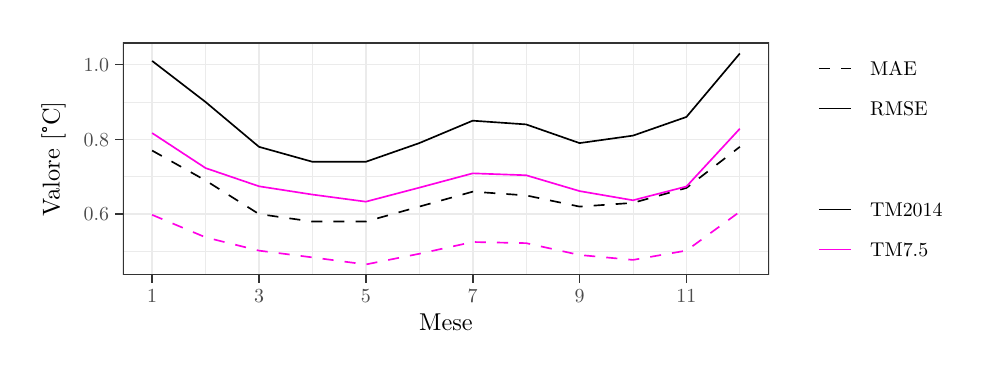
\begin{tikzpicture}[x=1pt,y=1pt]
\definecolor{fillColor}{RGB}{255,255,255}
\path[use as bounding box,fill=fillColor] (0,0) rectangle (341.43,116.66);
\begin{scope}
\path[clip] (  0.00,  0.00) rectangle (341.43,116.66);
\definecolor{drawColor}{RGB}{255,255,255}

\path[draw=drawColor,line width= 0.6pt,line join=round,line cap=round,fill=fillColor] (  0.00,  0.00) rectangle (341.43,116.66);
\end{scope}
\begin{scope}
\path[clip] ( 34.36, 27.29) rectangle (267.96,111.16);
\definecolor{fillColor}{RGB}{255,255,255}

\path[fill=fillColor] ( 34.36, 27.29) rectangle (267.96,111.16);
\definecolor{drawColor}{gray}{0.92}

\path[draw=drawColor,line width= 0.3pt,line join=round] ( 34.36, 35.80) --
	(267.96, 35.80);

\path[draw=drawColor,line width= 0.3pt,line join=round] ( 34.36, 62.80) --
	(267.96, 62.80);

\path[draw=drawColor,line width= 0.3pt,line join=round] ( 34.36, 89.80) --
	(267.96, 89.80);

\path[draw=drawColor,line width= 0.3pt,line join=round] ( 64.28, 27.29) --
	( 64.28,111.16);

\path[draw=drawColor,line width= 0.3pt,line join=round] (102.90, 27.29) --
	(102.90,111.16);

\path[draw=drawColor,line width= 0.3pt,line join=round] (141.51, 27.29) --
	(141.51,111.16);

\path[draw=drawColor,line width= 0.3pt,line join=round] (180.12, 27.29) --
	(180.12,111.16);

\path[draw=drawColor,line width= 0.3pt,line join=round] (218.73, 27.29) --
	(218.73,111.16);

\path[draw=drawColor,line width= 0.3pt,line join=round] (257.34, 27.29) --
	(257.34,111.16);

\path[draw=drawColor,line width= 0.6pt,line join=round] ( 34.36, 49.30) --
	(267.96, 49.30);

\path[draw=drawColor,line width= 0.6pt,line join=round] ( 34.36, 76.30) --
	(267.96, 76.30);

\path[draw=drawColor,line width= 0.6pt,line join=round] ( 34.36,103.29) --
	(267.96,103.29);

\path[draw=drawColor,line width= 0.6pt,line join=round] ( 44.98, 27.29) --
	( 44.98,111.16);

\path[draw=drawColor,line width= 0.6pt,line join=round] ( 83.59, 27.29) --
	( 83.59,111.16);

\path[draw=drawColor,line width= 0.6pt,line join=round] (122.20, 27.29) --
	(122.20,111.16);

\path[draw=drawColor,line width= 0.6pt,line join=round] (160.81, 27.29) --
	(160.81,111.16);

\path[draw=drawColor,line width= 0.6pt,line join=round] (199.43, 27.29) --
	(199.43,111.16);

\path[draw=drawColor,line width= 0.6pt,line join=round] (238.04, 27.29) --
	(238.04,111.16);
\definecolor{drawColor}{RGB}{0,0,0}

\path[draw=drawColor,line width= 0.6pt,dash pattern=on 4pt off 4pt ,line join=round] ( 44.98, 72.25) --
	( 64.28, 61.45) --
	( 83.59, 49.30) --
	(102.90, 46.60) --
	(122.20, 46.60) --
	(141.51, 52.00) --
	(160.81, 57.40) --
	(180.12, 56.05) --
	(199.43, 52.00) --
	(218.73, 53.35) --
	(238.04, 58.75) --
	(257.34, 73.60);

\path[draw=drawColor,line width= 0.6pt,line join=round] ( 44.98,104.64) --
	( 64.28, 89.80) --
	( 83.59, 73.60) --
	(102.90, 68.20) --
	(122.20, 68.20) --
	(141.51, 74.95) --
	(160.81, 83.05) --
	(180.12, 81.70) --
	(199.43, 74.95) --
	(218.73, 77.65) --
	(238.04, 84.40) --
	(257.34,107.34);
\definecolor{drawColor}{RGB}{255,0,230}

\path[draw=drawColor,line width= 0.6pt,dash pattern=on 4pt off 4pt ,line join=round] ( 44.98, 49.02) --
	( 64.28, 40.90) --
	( 83.59, 36.09) --
	(102.90, 33.65) --
	(122.20, 31.10) --
	(141.51, 34.96) --
	(160.81, 39.21) --
	(180.12, 38.80) --
	(199.43, 34.52) --
	(218.73, 32.74) --
	(238.04, 36.11) --
	(257.34, 50.16);

\path[draw=drawColor,line width= 0.6pt,line join=round] ( 44.98, 78.58) --
	( 64.28, 65.93) --
	( 83.59, 59.34) --
	(102.90, 56.35) --
	(122.20, 53.78) --
	(141.51, 58.85) --
	(160.81, 64.02) --
	(180.12, 63.33) --
	(199.43, 57.61) --
	(218.73, 54.29) --
	(238.04, 59.27) --
	(257.34, 80.16);
\definecolor{drawColor}{gray}{0.20}

\path[draw=drawColor,line width= 0.6pt,line join=round,line cap=round] ( 34.36, 27.29) rectangle (267.96,111.16);
\end{scope}
\begin{scope}
\path[clip] (  0.00,  0.00) rectangle (341.43,116.66);
\definecolor{drawColor}{gray}{0.30}

\node[text=drawColor,anchor=base east,inner sep=0pt, outer sep=0pt, scale=  0.72] at ( 29.41, 46.84) {0.6};

\node[text=drawColor,anchor=base east,inner sep=0pt, outer sep=0pt, scale=  0.72] at ( 29.41, 73.84) {0.8};

\node[text=drawColor,anchor=base east,inner sep=0pt, outer sep=0pt, scale=  0.72] at ( 29.41,100.83) {1.0};
\end{scope}
\begin{scope}
\path[clip] (  0.00,  0.00) rectangle (341.43,116.66);
\definecolor{drawColor}{gray}{0.20}

\path[draw=drawColor,line width= 0.6pt,line join=round] ( 31.61, 49.30) --
	( 34.36, 49.30);

\path[draw=drawColor,line width= 0.6pt,line join=round] ( 31.61, 76.30) --
	( 34.36, 76.30);

\path[draw=drawColor,line width= 0.6pt,line join=round] ( 31.61,103.29) --
	( 34.36,103.29);
\end{scope}
\begin{scope}
\path[clip] (  0.00,  0.00) rectangle (341.43,116.66);
\definecolor{drawColor}{gray}{0.20}

\path[draw=drawColor,line width= 0.6pt,line join=round] ( 44.98, 24.54) --
	( 44.98, 27.29);

\path[draw=drawColor,line width= 0.6pt,line join=round] ( 83.59, 24.54) --
	( 83.59, 27.29);

\path[draw=drawColor,line width= 0.6pt,line join=round] (122.20, 24.54) --
	(122.20, 27.29);

\path[draw=drawColor,line width= 0.6pt,line join=round] (160.81, 24.54) --
	(160.81, 27.29);

\path[draw=drawColor,line width= 0.6pt,line join=round] (199.43, 24.54) --
	(199.43, 27.29);

\path[draw=drawColor,line width= 0.6pt,line join=round] (238.04, 24.54) --
	(238.04, 27.29);
\end{scope}
\begin{scope}
\path[clip] (  0.00,  0.00) rectangle (341.43,116.66);
\definecolor{drawColor}{gray}{0.30}

\node[text=drawColor,anchor=base,inner sep=0pt, outer sep=0pt, scale=  0.72] at ( 44.98, 17.41) {1};

\node[text=drawColor,anchor=base,inner sep=0pt, outer sep=0pt, scale=  0.72] at ( 83.59, 17.41) {3};

\node[text=drawColor,anchor=base,inner sep=0pt, outer sep=0pt, scale=  0.72] at (122.20, 17.41) {5};

\node[text=drawColor,anchor=base,inner sep=0pt, outer sep=0pt, scale=  0.72] at (160.81, 17.41) {7};

\node[text=drawColor,anchor=base,inner sep=0pt, outer sep=0pt, scale=  0.72] at (199.43, 17.41) {9};

\node[text=drawColor,anchor=base,inner sep=0pt, outer sep=0pt, scale=  0.72] at (238.04, 17.41) {11};
\end{scope}
\begin{scope}
\path[clip] (  0.00,  0.00) rectangle (341.43,116.66);
\definecolor{drawColor}{RGB}{0,0,0}

\node[text=drawColor,anchor=base,inner sep=0pt, outer sep=0pt, scale=  0.88] at (151.16,  7.21) {Mese};
\end{scope}
\begin{scope}
\path[clip] (  0.00,  0.00) rectangle (341.43,116.66);
\definecolor{drawColor}{RGB}{0,0,0}

\node[text=drawColor,rotate= 90.00,anchor=base,inner sep=0pt, outer sep=0pt, scale=  0.88] at ( 11.56, 69.22) {Valore [\textdegree C]};
\end{scope}
\begin{scope}
\path[clip] (  0.00,  0.00) rectangle (341.43,116.66);
\definecolor{fillColor}{RGB}{255,255,255}

\path[fill=fillColor] (278.96, 74.72) rectangle (330.57,114.63);
\end{scope}
\begin{scope}
\path[clip] (  0.00,  0.00) rectangle (341.43,116.66);
\definecolor{fillColor}{RGB}{255,255,255}

\path[fill=fillColor] (284.46, 94.68) rectangle (298.92,109.13);
\end{scope}
\begin{scope}
\path[clip] (  0.00,  0.00) rectangle (341.43,116.66);
\definecolor{drawColor}{RGB}{0,0,0}

\path[draw=drawColor,line width= 0.6pt,dash pattern=on 4pt off 4pt ,line join=round] (285.91,101.90) -- (297.47,101.90);
\end{scope}
\begin{scope}
\path[clip] (  0.00,  0.00) rectangle (341.43,116.66);
\definecolor{fillColor}{RGB}{255,255,255}

\path[fill=fillColor] (284.46, 80.22) rectangle (298.92, 94.68);
\end{scope}
\begin{scope}
\path[clip] (  0.00,  0.00) rectangle (341.43,116.66);
\definecolor{drawColor}{RGB}{0,0,0}

\path[draw=drawColor,line width= 0.6pt,line join=round] (285.91, 87.45) -- (297.47, 87.45);
\end{scope}
\begin{scope}
\path[clip] (  0.00,  0.00) rectangle (341.43,116.66);
\definecolor{drawColor}{RGB}{0,0,0}

\node[text=drawColor,anchor=base west,inner sep=0pt, outer sep=0pt, scale=  0.72] at (304.42, 99.44) {MAE};
\end{scope}
\begin{scope}
\path[clip] (  0.00,  0.00) rectangle (341.43,116.66);
\definecolor{drawColor}{RGB}{0,0,0}

\node[text=drawColor,anchor=base west,inner sep=0pt, outer sep=0pt, scale=  0.72] at (304.42, 84.99) {RMSE};
\end{scope}
\begin{scope}
\path[clip] (  0.00,  0.00) rectangle (341.43,116.66);
\definecolor{fillColor}{RGB}{255,255,255}

\path[fill=fillColor] (278.96, 23.81) rectangle (335.93, 63.72);
\end{scope}
\begin{scope}
\path[clip] (  0.00,  0.00) rectangle (341.43,116.66);
\definecolor{fillColor}{RGB}{255,255,255}

\path[fill=fillColor] (284.46, 43.77) rectangle (298.92, 58.22);
\end{scope}
\begin{scope}
\path[clip] (  0.00,  0.00) rectangle (341.43,116.66);
\definecolor{drawColor}{RGB}{0,0,0}

\path[draw=drawColor,line width= 0.6pt,line join=round] (285.91, 51.00) -- (297.47, 51.00);
\end{scope}
\begin{scope}
\path[clip] (  0.00,  0.00) rectangle (341.43,116.66);
\definecolor{fillColor}{RGB}{255,255,255}

\path[fill=fillColor] (284.46, 29.31) rectangle (298.92, 43.77);
\end{scope}
\begin{scope}
\path[clip] (  0.00,  0.00) rectangle (341.43,116.66);
\definecolor{drawColor}{RGB}{255,0,230}

\path[draw=drawColor,line width= 0.6pt,line join=round] (285.91, 36.54) -- (297.47, 36.54);
\end{scope}
\begin{scope}
\path[clip] (  0.00,  0.00) rectangle (341.43,116.66);
\definecolor{drawColor}{RGB}{0,0,0}

\node[text=drawColor,anchor=base west,inner sep=0pt, outer sep=0pt, scale=  0.72] at (304.42, 48.53) {TM2014};
\end{scope}
\begin{scope}
\path[clip] (  0.00,  0.00) rectangle (341.43,116.66);
\definecolor{drawColor}{RGB}{0,0,0}

\node[text=drawColor,anchor=base west,inner sep=0pt, outer sep=0pt, scale=  0.72] at (304.42, 34.08) {TM7.5};
\end{scope}
\end{tikzpicture}
